\documentclass[10pt,a4paper]{article}
\usepackage[utf8]{inputenc}
\usepackage{amsmath}
\usepackage{amsfonts}
\usepackage{amssymb}
\usepackage{graphicx}
\usepackage{todo}
\author{Christoph Robbert 6577945, Peter Stilow 6500440}
\title{Protokoll 0}
\begin{document}
\maketitle
 
\section{Aufgabe 1}
Nach einem Login auf den Rechner \texttt{cultofthedeadcow.seclab.uni-paderborn.de/192.26.175.11} sah man an der Ausgabe von \texttt{ifconfig}, dass sich dieser Rechner im Subnetz \texttt{192.26.175.0/26} befand.
Ein Anschließender Pingscan mittels \texttt{nmap -sP 192.26.175.0/26} zeigte, dass die Hosts aus Figure \ref{0_netlayout} in diesem Subnetz erreichbar sind.
Außerdem zeigte ein anschließender Portscan( \texttt{nmap -sT -sV} die folgenden offenen Ports:
\begin{figure}
\label{0_netlayout}
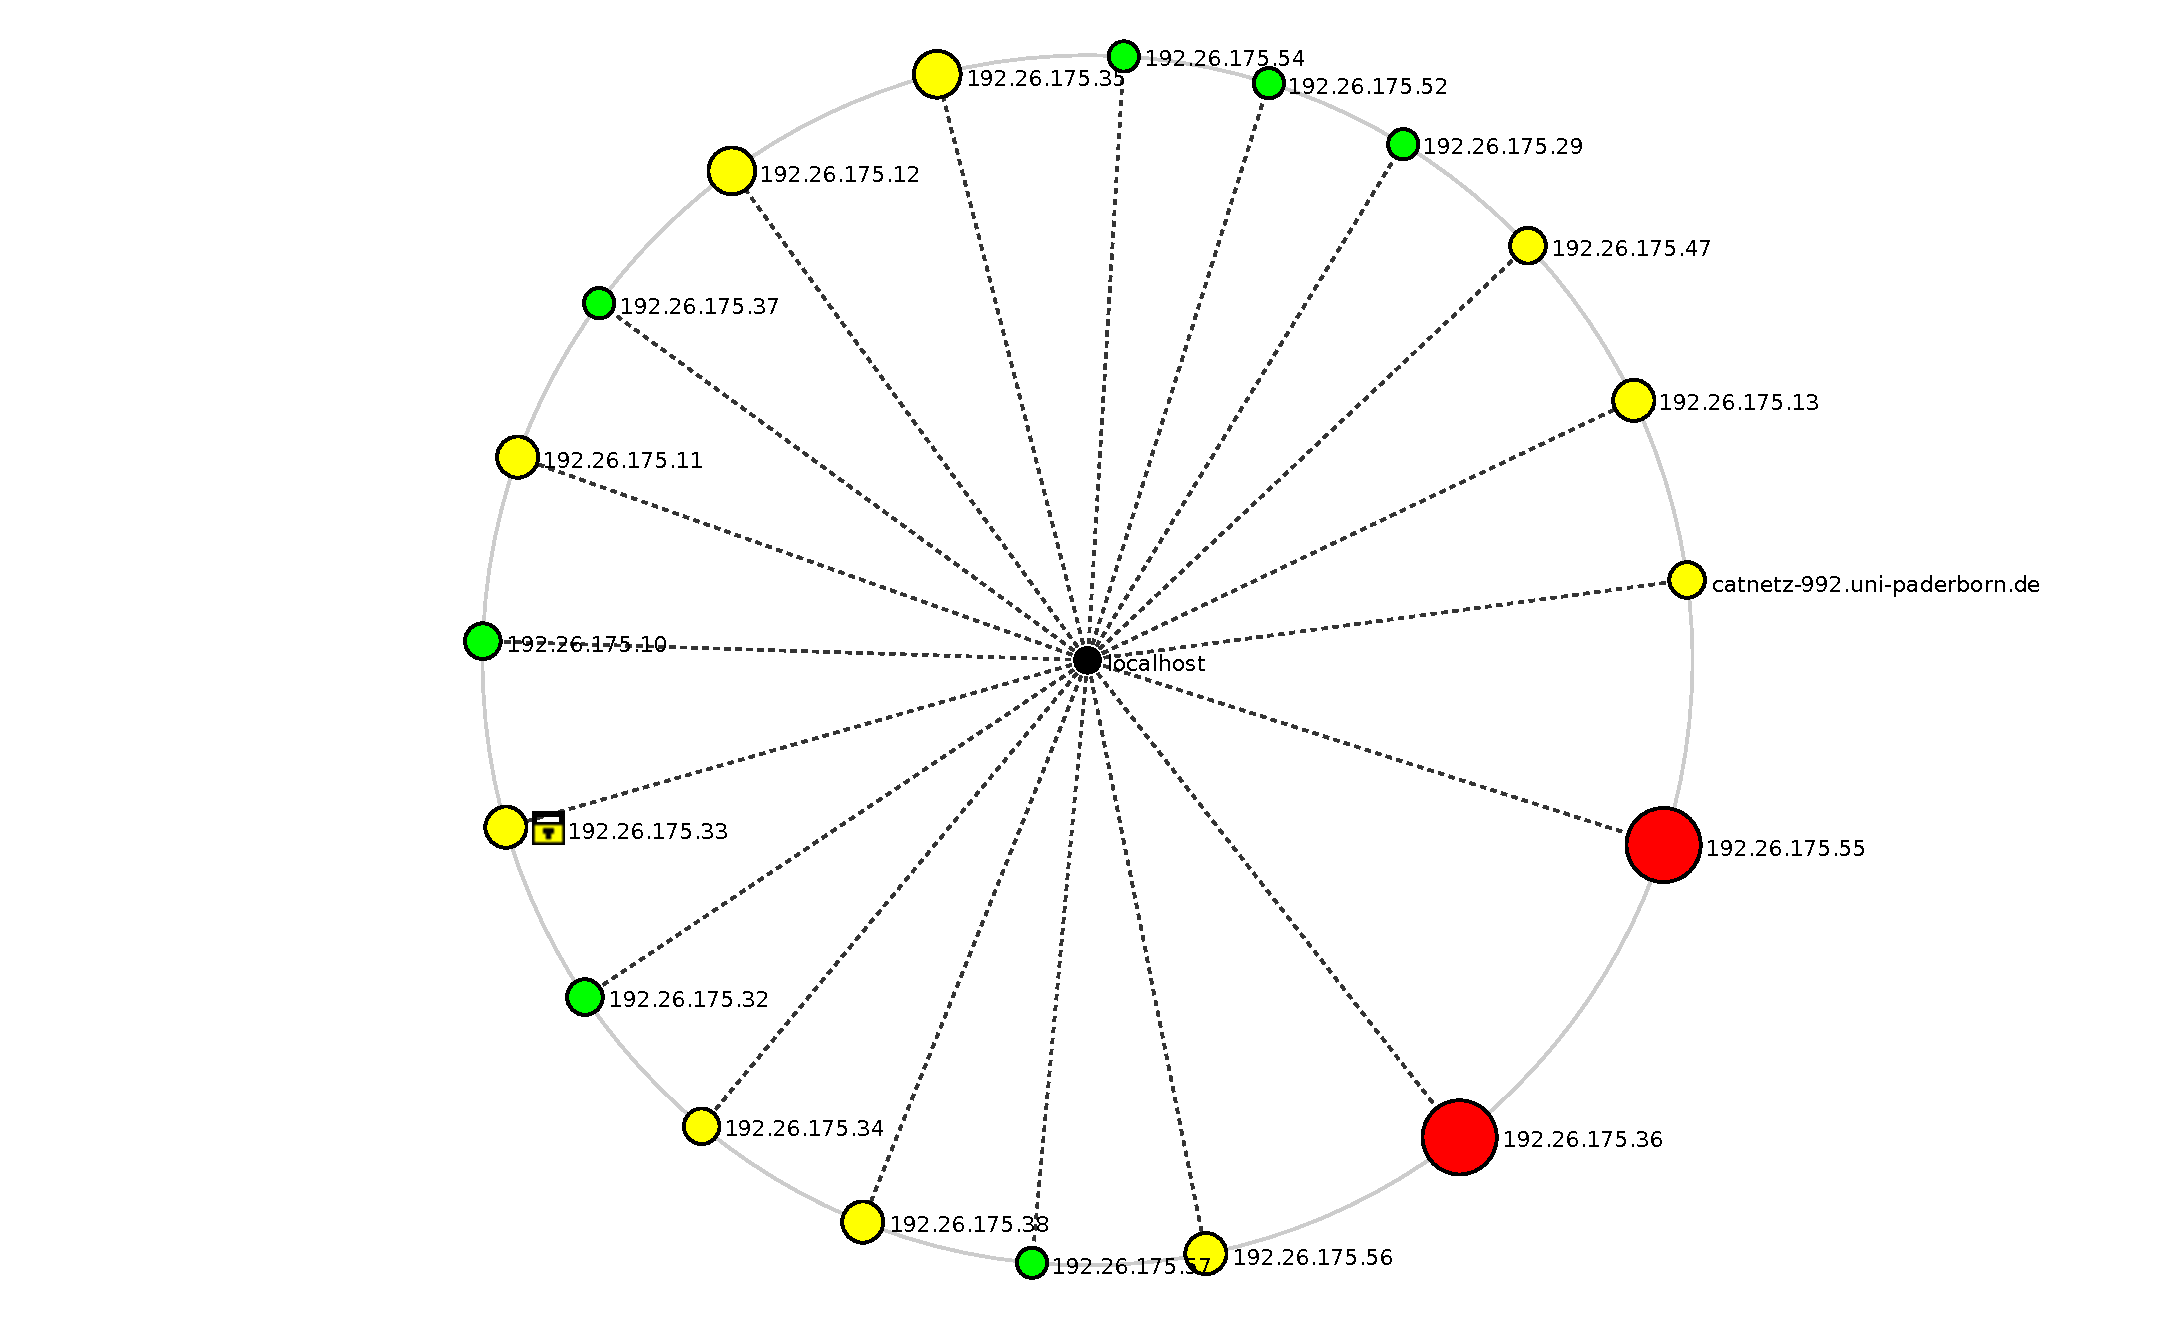
\includegraphics[scale=0.4]{figures/0_netlayout.pdf}
\caption{Struktur des Netzes im Security Lab.}
\end{figure}
\begin{itemize}
\item catnetz-992.uni-paderborn.de (192.26.175.1)
\begin{verbatim}
22/tcp  open  ssh      Cisco SSH 1.25 (protocol 1.99)
80/tcp  open  http     Cisco IOS administrative httpd
443/tcp open  ssl/http Cisco IOS administrative httpd
Service Info: OS: IOS
\end{verbatim}
Aus den Angaben des Portscan lässt sich schließen, dass es sich um einen Cisco Router handelt bei diesem Host. Da die Automatische Dienstanalyse von \texttt{nmap} sowohl bei den Diensten Cisco Dienste identifiziert alsauch bei der Service Info das Routerbetriebssystem IOS. 
\item 192.26.175.10
\begin{verbatim}
22/tcp  open  ssh     OpenSSH 5.9p1 Debian 5ubuntu1 (protocol 2.0)
111/tcp open  rpcbind
Service Info: OS: Linux
\end{verbatim}
Bei diesem Host wird es sich um einen Ubuntu 12.04 Rechner handeln. Dies schließen wir aus dem Versionsstring '5ubuntu1', da diese Version des openssh Servers nur in Ubuntu 12.04 verwendet wurde. Außer dem ssh und dem rpcbind Dienst wurde kein Dienst auf diesem Server identifiziert.
\item cultofthedeadcow.seclab.uni-paderborn.de (192.26.175.11)
\begin{verbatim}
22/tcp   open  ssh           OpenSSH 5.9p1 Debian 5ubuntu1.1 (protocol 2.0)
111/tcp  open  rpcbind
3389/tcp open  microsoft-rdp xrdp
8080/tcp open  http          Apache Tomcat/Coyote JSP engine 1.1
Service Info: OS: Linux
\end{verbatim}
Dieser Rechner ist ein Ubuntu 12.04.3 Rechner. Da Zugang zu diesem Rechner per SSH besteht kann man via \texttt{vim /etc/issue} diese Versionbezeichung eindeutig bestimmen. Neben dem schon bekannten SSH Dienst läuft auch ein rpcbind Dienst, ein Apache Tomcat Anwendungsserver und der microsoft-rdp Dienst für RemoteDesktopverbindungen.
\item 192.26.175.12
\begin{verbatim}
22/tcp   open  ssh           OpenSSH 5.9p1 Debian 5ubuntu1.1 (protocol 2.0)
111/tcp  open  rpcbind
3389/tcp open  microsoft-rdp xrdp
5910/tcp open  vnc           VNC (protocol 3.3; Locked out)
Service Info: OS: Linux
\end{verbatim}
Dieser Rechner scheint auch ein Ubuntu 12.04 Rechner zu sein. Neben dem openssh Server und dem rpcbind Dienst scheint auch ein microsoft-rdp Dienst und ein VNC Dienst für Remotelogins aktiv zu sein.
\item 192.26.175.13
Der Portscan brachte dieselben Ergebnisse wie beim Rechner mit der IP 192.26.175.11
\item 192.26.175.14
Der Portscan brachte dieselben Ergebnisse wie beim Rechner mit der IP 192.26.175.12
\item 192.26.175.29
\begin{verbatim}
139/tcp open  netbios-ssn
137/udp open|filtered netbios-ns
138/udp open|filtered netbios-dgm
\end{verbatim}
Da hier der netbios Dienst läuft, schließen wir, dass es sich um einen Windows Rechner handelt. Die genaue Version ist Aufgrund der Portscans nicht zu ermitteln.
\item 192.26.175.32
\begin{verbatim}
22/tcp open  ssh     OpenSSH 5.8p2_hpn13v11 (FreeBSD 20110503; protocol 2.0)
25/tcp open  smtp
\end{verbatim}
Bei diesem Rechner wird es sich laut der verwendeten OpenSSH Serverversion um einen FreeBSD Rechner handeln. Neben dem OpenSSH Server läuft auch ein smtp Server(E-Mailannehmender Server). 
\item 192.26.175.33
\item 192.26.175.34
\item 192.26.175.35
\item 192.26.175.36
\item 192.26.175.37
\item 192.26.175.38
\item 192.26.175.47
\item 192.26.175.49
\item 192.26.175.54
\item 192.26.175.55
\item 192.26.175.56
\end{itemize}

\section{Aufgabe 2}
\begin{description}
	\item[flgbab8e275f92ee6cf9fd48333dfeb0b85] Beim Aufstellen der Stützen unter der Tastatur fiel dieser Hardwareflag auf. 
	\item[flgbb315509cf9c5caac09624d258c3d95d] Beim einloggen via \texttt{ssh} auf den Rechner \texttt{192.26.175.11} und anschließendem "orientieren" via \texttt{ls} fiel auf, dass ein Windowsbatch mit dem Namen \texttt{runme.bat} auf einem Linuxsystem erstellt wurde. Um zu schauen was es damit aufsich hat, begutachteten wir den Inhalt des Skriptes mittels \texttt{vim}. Das Skript gibt via \texttt{echo} den String dieses Flags aus.
	Außerdem fanden wir dieses Flag auf dem FTP Server auf dem Rechner \texttt{192.26.175.38} in der Datei \\ \texttt{/follow/the/white/rabbit/runme.bat}
	\item[flg58594831dfbe63560f940365d517fa68] Zum finden dieses Flags haben wir mit Wireshark im Capture Mode einfach alle Packete im Netzwerk abgefangen. Dabei fiel dieses Flag in einen UDP Packet vom Rechner 192.26.175.36 zum Rechner 192.26.175.63 auf.
	\item[flg8e7fa2f4b3e3390175badcc38141bd1f] Auf dem Rechner \texttt{192.26.175.35} läuft ein FTP-Server. Beim Durchsuchen der Inhalte fiel eine Datei auf, in der der Benutzer Bernd dazu aufgefordert wurde ein Passwort für sein MySQL Account zu setzen. Da auf demselben Rechner ein MySQL Server lief, loggten wir uns als Benutzer \texttt{bernd} auf diesem MySQL Server ein. In der Datenbank \texttt{bernd} fanden wir die Tabelle \texttt{hier\_gibts\_aktuelle\_flags}. Ein \texttt{select * from hier\_gibts\_aktuelle\_flags;} brachte das obengenannte Flag zu Tage.
	\item[flg0607547c0d12497a21ab8a0b53dd5bed] Auf dem Rechner \texttt{192.26.175.35} läuft auch ein HTTP-Server. Beim Aufrufen der URL \texttt{http://192.26.175.35} fanden wir im HTML-Quelltext der angezeigten Website dieses Flag. Es war im Webbrowser nicht zu sehen, da es auskommentiert wurde im HTML Quellcode.
	\item[flgd0d1741e939d8fc51e0dae50ff39bed4] Beim Scannen des Rechners \texttt{192.26.175.35} mit dem nmap Kommando \texttt{nmap -T4 -A -v 192.26.175.35} viel als UFT8 Servername im Dienst Netatalk dieses Flag auf.
\end{description}

\end{document}